\documentclass{report}
\usepackage[utf8]{inputenc}
\usepackage{graphicx}
\usepackage{multirow}
\usepackage{caption}
\usepackage{subcaption}
\usepackage{amsfonts}
\usepackage{multicol}
\usepackage{listings}
\lstset{
  basicstyle=\ttfamily,
  mathescape
}
\usepackage[utf8]{inputenc}
\usepackage[spanish]{babel}
\usepackage{lscape}
\usepackage[left=1.5cm,right=1.5cm,top=2cm,bottom=2cm]{geometry}

\begin{document}

\begin{center}
    
    \begin{tabular}{l c r}
    
\includegraphics[scale=0.15]{Imagenes/IPN.jpeg}
    & 
        \bf\fontsize{22}{0}{\selectfont{Instituto Polit\'ecnico Nacional}}

    
    & 
\includegraphics[scale=0.08]{Imagenes/escom.png} \\
     
    & \bf\fontsize{22}{0}{\selectfont{ Escuela Superior de C\'omputo}} &  \\
    \end{tabular}

    
    \vspace*{2\baselineskip}
    
    {
        \bf\fontsize{12}{0}{\selectfont{An\'alisis de Algoritmos, Sem: 2021-1, 3CV1, Pr\'actica 2, 26/10/20}}
    }
            
    \vspace*{2\baselineskip}
             
    {
        \fontsize{23}{0}{\selectfont{Práctica 2: Funciones Recursivas vs Iterativas}}
    }
    
    \vspace*{2\baselineskip}
    
    {
        \bf\fontsize{12}{0}{\selectfont{Valle Mart\'inez Luis Eduardo, Rivero Ronquillo Omar Imanol}}
    }
    
    \vspace*{1\baselineskip}
    
    {
        \fontsize{12}{0}{\textit{lvalle212@gmail.com, imanol.rivero7@gmail.com}}
    }
    
    \vspace*{2\baselineskip}

    {
        \fontsize{12}{0}\selectfont{
        \textbf{Resumen:} En el presente documento se presenta una comparación del análisis de los algoritmo recursivos frente a los iterativos}
        
        \fontsize{12}{0}\selectfont{
        \textbf{Palabras Clave:} Algoritmo iterativos, Algoritmos Recursivos, Java.}
    
    }
\end{center}

\hfill \break
\hfill \break
\hfill \break

\section*{Introducción} 
    En el area de las ciencias de la computaci\'on se tiene una gran diversidad de algoritmos. Estos pueden ser clasificados con patrones bien definidos que los distinguen unos de otros.\\
    Los algoritmos iterativos se caracterizan por ejecutarse mediante ciclos. Este tipo de algoritmos son muy \'utiles al momento de realizar tareas repetitivas. Por otro lado, los algoritmos recursivos son aquellos que buscan resolver un problema sustituy\'endolo por otros problemas de la misma categoria, pero m\'as simples. Se dice que un algoritmo es recursivo si dentro del cuerpo del algoritmo y de forma directa o indirecta se realiza una llamada a s\'i mismo.\\
    Para esta pr\'actica se desarrolla un analisis de complejidad de los algoritmos propuestos, comprobando de forma analitica y de forma experimental la eficiencia de los algorimos en cuesti\'on.
\section*{Conceptos B\'asicos}
    Método de sustitución hacia atrás
    
    Se realizará el análisis de 3 algoritmos diferentes, que toman enfoques distintos para otorgar el mismo resultado.
    La primer tercia, realiza el producto de 2 números enteros:
    \subsection*{Producto de 2 enteros}
    Los 3 algoritmos reciben como argumento a los 2 enteros y regresan el valor del producto también como un entero.\\
        \subsubsection*{Prod1}
            De naturaleza iterativa, el algoritmo \textbf{prod1} realiza \textit{n} veces la suma de \textit{m} mediante un bucle while que por cada iteración disminuirá en la unidad el valor de \textit{n} hasta que sea 0.
            \begin{verbatim}
                int prod1(m,n)
                    r=0
                    while n>0
                        r = r+m
                        n--
                    return r
            \end{verbatim}
            \begin{itemize}
                \item\textbf{¿Cu\'ando se obtiene el mejor caso?}\\
                Este caso lo encontramos cuando $n \leq 0$ ya que solo verifica la condici\'on del bloque while una sola vez sin ejecutar su contenido.
                \item\textbf{¿Cu\'ando se obtiene el peor caso?}
                Para este algoritmo, no se encuentra un peor caso, pero un caso general que se obtiene cuando $n > 0$ incrementando los pasos que tiene que ejecutar creciendo de forma lineal según sea el valor de $n$.
                \item\textbf{C\'alculo anal\'itico de orden de complejidad}
                \begin{verbatim}
                int prod1(m,n)
                    r=0             C1    |   1
                    while n>0       C2    |   n+1
                        r = r+m     C3    |   n     
                        n--         C4    |   n
                    return r        C5    |   1
                \end{verbatim}
                Luego,\\\\$T(n) = C_{1}+C_{2}(n+1)+C_{3}n+C_{4}n+C_{5} = C_{1}+C_{2}n+C_{2}+C_{3}n+C_{4}n+C_{5} = (C_{2}+C_{3}+C_{4})n+(C_{1}+C_{2}+C_{5})$\\\\
                Entonces, nuestra $T(n)$ es de la forma $an+b$. Por lo que el mejor caso tendrá una complejidad constante: $ T(n) \in \Omega(n)$\\
                Para el caso general, tendremos la complejidad lineal: $ T(n) \in \Theta(n)$
            \end{itemize}
            
        \subsubsection*{Prod2}
            Otro algoritmo de naturaleza iterativa. Funciona dentro de un ciclo while que se ejecuta mientras \textit{n} sea mayor a 0. Para lograr que el algoritmo funcione, es necesario ocupar únicamente la parte entera de las operaciones que requieren división.\\
            
            Se va a multiplicar el valor de \textit{m} por una potencia de 2, que dependerá del número de la iteración dentro del ciclo. De esta forma, el valor de \textit{m}:\\
            Para la primer iteración
            $$m = 2^1 * m$$\\
            Para la segunda iteración
            $$m = 2^2 * m$$
            ...\\
            Entonces para la \textit{k} iteración
            $$m = 2^k * m$$\\
            
            Donde \textit{k} se defina a partir de \textit{n}:
            $$\frac{n}{2^k} = 1$$
            $$2^k=n$$
            $$klog(2)=log(n)$$
            $$k=log(n)$$\\
            
            Mientras \textit{n} será decrementada al ser dividida por un potencia de 2 en cada iteración.\\
            
            Para obtener el producto resultante, se realiza la condición mediante una comparación a nivel bit de \textit{n} con 1 ($n\&1$), resultando cierta la condición cuando el valor de \textit{n} es impar, así el valor que conserva \textit{m} de la iteración pasada se irá sumando a la variable auxiliar \textit{r}.
            \begin{verbatim}
                int prod2(m,n)
                    r=0
                    while n>0
                        if n & 1
                            r = r+m
                        m = 2*m
                        n = n/2
                    return r
            \end{verbatim}
            \begin{itemize}
                \item\textbf{¿Cu\'ando se obtiene el mejor caso?}\\
                Corresponde al caso en que $n\leq 0$, ya que en este caso tampoco ejecutaria el contenido del while, devolviendo directamente $r=0$.
                \item\textbf{¿Cu\'ando se obtiene el peor caso?}\\
                El peor caso puede ser considerado como aquel que es el general para este alogoritmo en particular.Se obtendrá el caso general cuando el valor de $n>0$ 
                \item\textbf{C\'alculo anal\'itico de orden de complejidad}
                \begin{verbatim}
                int prod2(m,n)
                    r=0                 C1 | 1
                    while n>0           C2 | k = log(n)+1
                        if n & 1        C3 | log(n)
                            r = r+m     C4 | constante
                        m = 2*m         C5 | log(n)
                        n = n/2         C6 | log(n)
                    return r            C7 | 1
                \end{verbatim}
                Luego,\\\\ $T(n) = C_{1}+C_{2}(log(n)+1)+C_{3}log(n)+C_{4}+C_{5}log(n)+C_{6}log(n)+C_{7}=Clog(n)+C$\\\\
                De esta forma obtenemos para el mejor caso un complejidad constante: $T(n) \in \Omega(1)$\\
                Y en el caso promedio una complejidad logarítmica: $T(n) \in \Theta(log(n))$ \\
            \end{itemize}
            
        \subsubsection*{Prod3}
            El último de los algoritmos para obtener el producto de 2 números enteros, ser\'a recursivo.\\
            
            La lógica detrás de este algoritmo es igual a la de \textbf{prod1}, donde se irá sumando \textit{b} veces el número \textit{a}. 
            
            El caso base para esta recursión es cuando \textbf{b} es igual a 1, por lo que solamente se regresa el valor de \textit{a}. En caso contrario, al valor de \textit{a} se le deberá sumar el valor de la función con \textit{b-1}.
            \begin{verbatim}
                int prod3(a,b)
                    if b =1
                        return a
                    else
                        return a+prod3(a,b-1)
            \end{verbatim}
            \begin{itemize}
                \item\textbf{¿Cu\'ando se obtiene el mejor caso?}\\
                Le corresponde al caso en que nuestra variable de entrada a la primera iteraci\'on es $b=1$.
                \item\textbf{¿Cu\'ando se obtiene el peor caso?}\\
                Este se obtiene cuando encontramos desde la primera iteraci\'on un $b>a$ que aumenta las veces que vuelve a ejecutar el algoritmo recursivo sin importar si desde el inicio la primera iteraci\'on tiene  $a=0$. Adem\'as no se considera el caso en que directamente $b=0$.
                \item\textbf{C\'alculo anal\'itico de orden de complejidad}
                Del algoritmo obtenemos la condición base y el caso general:
                \begin{center}
                    $prod3(a,b) = 
                    \left\{
                        \begin{array}{lcc}
                            a & si & b=1\\
                            a+prod3(a,b-1) & si & otro
                        \end{array}
                    \right.$
                \end{center}
                Sea $M(n)$ el n\'umero de sumas que realiza $prod3(a,b)$ para calcular el producto final. Entonces:
                \begin{center}
                    $M(n)=M(n-1)+1$
                \end{center}
                Ya que se requieren $M(n-1)$ sumas para calcular $prod3(a,b-1)$ y una más para sumar con $a$. Adem\'as $M(0)=a$ ya que no se ejecuta ninguna suma. Por lo tanto nuestra ecuaci\'on de recurrencia para este algoritmo, se define como:
                \begin{center}
                    $M(n) = 
                    \left\{
                        \begin{array}{lcc}
                            1 & si & n=0\\
                            M(n-1)+1 & si & n>0
                        \end{array}
                    \right.$
                \end{center}
                Resolviendo mediante el m\'etodo de sustituci\'on hacia atr\'as. Se tiene:
                \begin{multicols}{2}{}
                Si $n>0$\\
                    $M(n)=M(n-1)+1$\\
                    $=M(n-2)+2$\\
                    $=M(n-3)+3$\\
                    ...\\
                    ...\\
                    ...\\
                    Para i, $=M(n-i)+i$\\
                    ...\\
                    ...\\
                    Nos detenemos cuando $n-i=0$, entonces
                    $n=i$\\
                    $=M(0)+n$\\
                    $=n$\\
                    $\Rightarrow M(n)\in\Theta(n)$
                \end{multicols}
            \end{itemize}
    \subsection*{Cociente de 2 enteros}
        Se tiene ahora, una tercia de algoritmos que calculan el cociente de 2 números enteros.
        \subsubsection*{Div1}
            El primer algoritmo, ser\'a una solución iterativa al problema. Se aceptan ahora 3 argumentos de la función, el primero será el entero dividendo(\textit{n}), el segundo el divisor(\textit{div}) y el último será un apuntador para poder obtener el residuo(\textit{r}).
            
            Este parte del principio que la división es la operación inversa de la multiplicación, por lo que ahora en vez de realizar sumas, se debera restar.\\
            
            Se ejecuta dentro de un bucle while, que iterará hasta que el valor de \textit{n} sea menor al de \textit{div}(divisor). En cada iteración, se restara 1 vez \textit{div} de \textit{n}, y al cociente, representado por \textit{q}, se le sumará la unidad.\\
            
            Al final del ciclo, al apuntador \textit{r} se le asigna el valor de n, es decir, el valor restante de la división o residuo.
            \begin{verbatim}
                int div1(n,div,*r)
                    q = 0
                    while n>=div
                        n=n-div
                        q++
                    *r = n
                    return q
            \end{verbatim}
            \begin{itemize}
                \item\textbf{¿Cu\'ando se obtiene el mejor caso?}\\
                Se distingue como mejor caso, a las entradas donde el divisor \textit{div} será mayor que el dividendo \textit{n}, evitando la ejecución de las lineas dentro del while,tan solo se realizará la comprobaci\'on del ciclo while en una ocasi\'on.
                \item\textbf{¿Cu\'ando se obtiene el peor caso?}\\
                El peor caso será cuando el divisor \textit{div}, sea ingresado con el valor de 1.
                \item\textbf{C\'alculo anal\'itico de orden de complejidad}\\
                Ahora se realizar\'a el c\'alculo de complejidad considerando el orden de complejidad por linea.
                \begin{lstlisting}
                    int div1(n,div,*r)
                        q = 0           $\mathcal{O}(1)$
                        while n>=div    $\mathcal{O}(n)$
                            n=n-div     $\mathcal{O}(1)$          
                            q++         $\mathcal{O}(1)$
                        *r = n          $\mathcal{O}(1)$
                    return q            $\mathcal{O}(1)$
                \end{lstlisting}
                Se observa que el número de veces que se ejecuta el bucle while corresponde con el valor de \textit{q}, más no nos es útil la variable a retornar para analizar la ejecución del bucle. Se plantea la siguiente ecuación donde el valor derecho de la igualdad debería llegar a ser menor al valor de \textit{div}:
                $$div = n - kdiv$$
                $$div-n = -kdiv$$
                $$k=\frac{n-div}{div}$$
                Donde será \textit{k} el número de iteraciones que se realizan hasta que \textit{n} tome el valor de \textit{div}, y para poder terminar la ejecución se le suma 1 a \textit{k}, quedándo finalmente como:
                $$k = \frac{n-div}{div}+1$$\\
                Para el peor caso se va considerar el valor de \textit{div} como 1, por tal razón vamos a obtener una complejidad $O(n)$.
                Ésta será la complejidad m\'axima de las líneas conformando a la función, de tal manera que finalmente $T(n)\in O(n)$.
            \end{itemize}
            
        \subsubsection*{Div2}
            El segundo algoritmo para obtener el cociente también será recursivo y tendrá los mismos argumento de función que el primero.\\
            
            Este en cambio, iniciará asignando de entrada el residuo con el valor de \textit{n}, y a una variable auxilir \textit{dd}, que tomará el valor de \textit{div}.
            
            Se inicia el primer ciclo de iteraciones que cambiará el valor de \textit{dd} al multiplicarlo por una potencia de 2 $dd = 2^j dd$, se apunta que el valor de \textit{dd} se obtiene del argumento de función \textit{div}, permitiéndonos sustituir la en la ecuación cuando el valor sea igual a \textit{n}:
            $2^j * div = n$
            $j=log(\frac{n}{div})$
            En la ecuación, \textit{j} será el número de iteraciones, y a este resultado, se le sumará 1 por la última iteración que se realiza cuando \textit{dd} sigue siendo menor o igual a \textit{n}, pero que al final del bucle lo volverá mayor a \textit{n}.\\
            
            En el segundo bucle se inicia el procedimiento para el cálculo del cociente. Este bucle iterará mientras el valor calculado anteriormente de \textit{dd} sea mayor al del divisor(\textit{div}). Para esto, \textit{dd} será dividido por una potencia de 2, como proceso inverso, y \textit{q} también será multiplicado por la misma potencia de 2, pero su valor ira cambiando según el condicionamiento dentro del bucle.\\
            
            La condición restará el valor de \textit{dd} al residuo \textit{r}, y se aumenta en la unidad el cociente.
            
            Finalmente, el número de iteraciones que realiza, al ser un proceso inverso, en lo que respecta al cambio de los valores de \textit{dd}, seguirá siendo $j=log(\frac{n}{div})$
            \begin{verbatim}
                int div2(n,div,*r)
                    dd = div
                    q = 0
                    *r = n
                    while dd<=n
                        dd = 2*dd
                    while dd>div
                        dd = dd/2
                        q = 2*q
                        if dd <= *r
                            *r = *r-dd
                            q++
                    return q
            \end{verbatim}
            \begin{itemize}
                \item\textbf{¿Cu\'ando se obtiene el mejor caso?}\\
                El mejor caso, al igual que con \textit{div1}, será cuando el divisor \textit{div}, es mayor al dividendo \textit{n}.
                \item\textbf{¿Cu\'ando se obtiene el peor caso?}\\
                El peor caso para este algoritmo lo encontramos cuando $div=1$. con esta configuración de valores, se ejecutaria más veces las restas para cualquier valor de n.
                \item\textbf{C\'alculo anal\'itico de orden de complejidad}\\
                Para el cálculo de la complejidad de este algoritmo, consideramos las ecuaciones explicadas anteriormente, y rescatamos la ecuación $j = log(\frac{n}{div})$ que expone la complejidad del primer bucle, se transcribe de la siguiente manera: $\Theta(log(\frac{n}{div}))$, pero la complejidad es una función que depende de la variable \textit{n} y \textit{div} se considera constante, quedándonos simplemente: $$\Theta(log(n))$$
                \begin{lstlisting}
                    dd = div            $\mathcal{O}(1)$
                    q = 0               $\mathcal{O}(1)$
                    *r = n              $\mathcal{O}(1)$
                    while dd<=n         $\mathcal{O}(log (n))$
                        dd = 2*dd       $\mathcal{O}(1)$
                    while dd>div        $\mathcal{O}(log(n))$
                        dd = dd/2       $\mathcal{O}(1)$
                        q = 2*q         $\mathcal{O}(1)$
                        if dd <= *r     $\mathcal{O}(1)$
                            *r = *r-dd  $\mathcal{O}(1)$
                            q++         $\mathcal{O}(1)$
                    return q            $\mathcal{O}(1)$
                \end{lstlisting}
            \end{itemize}\\
            Siendo $\Theta(log(n))$ la complejidad mayor, la función tendrá complejidad $T(n) \in \Theta(log(n))$
        
        \subsubsection*{Div3}
            El último algoritmo de la tercia ser\'a el de naturaleza recursiva. Este algoritmo también aplicará la lógica de \textbf{div1}, donde se suman las veces que \textit{div} puede restársele a n.
            
            A diferencia de los algoritmo anteriores, este solo dispone de 2 argumentos de función, \textit{n} o dividendo, y \textit{div} o divisor, por lo que no se conoce el residuo al terminar la función, pero que facilmente podría incorporársele para conocerlo.\\
            
            El caso base para esta recursión es cuando el valor del divisor es mayor que \textit{n}, por lo que el valor actual de n será ya el residuo y por lo tanto no se le suma la unidad al cociente, más se regresa el valor 0. En caso contrario, se sumará la unidad al resultado de la misma función para los valores del dividendo menos el divisor: $div3(n-div,div)$.
            \begin{verbatim}
                int div3(n,div)
                    if div>n
                        return 0
                    else
                        return 1+div3(n-div,div)
            \end{verbatim}
            \begin{itemize}
                \item\textbf{¿Cu\'ando se obtiene el mejor caso?}\\
                El mejor caso lo encontramos cuando el divisor \textit{div} es mayor a \textit{n}. Ya que evitamos el mayor numero de lineas con este valor como entrada.
                \item\textbf{¿Cu\'ando se obtiene el peor caso?}\\
                Al igual que en los algoritmo anteriores, el peor caso para este algoritmo será cuando el divisor es igual a 1, asegurando para cualquier valor de \textit{n} el mayor número de restas posible.
                \item\textbf{C\'alculo anal\'itico de orden de complejidad}
                Del algoritmo obtenemos la condición base y el caso general:
                \begin{center}
                    $div3(n,div) = 
                    \left\{
                        \begin{array}{lcc}
                            0 & si & div>n\\
                            1+div3(n-div,div) & si & otro
                        \end{array}
                    \right.$
                \end{center}
                Sea $M(n)$ el n\'umero de sumas que realiza $div3(a,b)$ para calcular el cociente final. Entonces:
                \begin{center} 
                    $M(n)=M(n-div)+1$
                \end{center}
                Ya que se requieren $M(n-div)$ sumas, con \textit{div} constante, para calcular $div3(n-div,div)$ y una más para sumar con $1$. Adem\'as $M(0)=1$ ya que no se ejecuta ninguna suma. Por lo tanto nuestra ecuaci\'on de recurrencia para este algoritmo, se define como:
                \begin{center}
                    $M(n) = 
                    \left\{
                        \begin{array}{lcc}
                            1 & si & n<div
                            \\
                            M(n-1)+1 & si & otro
                        \end{array}
                    \right.$\\
                \end{center}
                Ahora, considerando para $n>1$\\
                    $M(n)=M(n-1)+1+\mathcal{O}(1)$\\
                    $M(n)=M(n-1)+\mathcal{O}(1)$\\
                    $M(n)=M(n-1)+C$, siendo c una constante.\\\\
                Resolviendo mediante el m\'etodo de sustituci\'on hacia atr\'as. Se tiene:
                \begin{multicols}{2}{}
                    $M(n)=M(n-1)+C$\\
                    $=M(n-2)+2C$\\
                    $=M(n-3)+3C$\\
                    ...\\
                    ...\\
                    ...\\
                    Para i, $=M(n-i)+iC$\\
                    ...\\
                    ...\\
                    Nos detenemos cuando $n-i=0$, entonces
                    $n=i$\\
                    $=M(0)+nC = C+nC$\\
                    Por lo tanto, $M(n)\in\mathcal{O}(n)$\\
                \end{multicols}
            \end{itemize}

\newpage

\section*{Experimentación y Resultados}
    \subsection*{Producto 3 enteros}
        A continuación se muestran las gráficas generadas de los pares ordenadas que corresponden al valor de la \textit{n}, eje de las abscisas, y el tiempo de procesamiento \textit{t} en $\mu$ seg, para cada uno de los 3 algoritmos del producto de 2 números enteros.\\
        \subsubsection*{Gráficas de tamaño vs tiempo}
                
            \begin{figure}[!h]
                \centering
                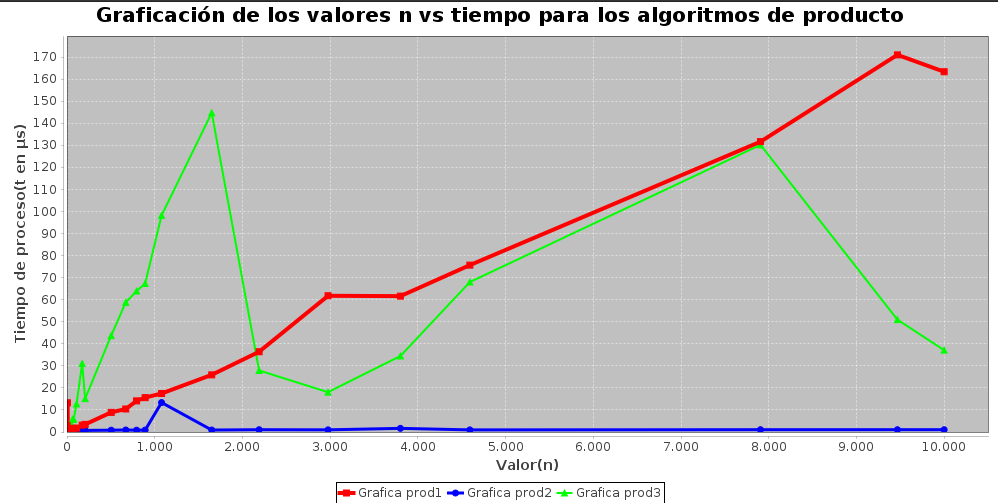
\includegraphics[width=20cm]{Imagenes/ResultadosExperimentalesProductos.png}
                \caption{Gráficas de los puntos ordenados obtenidos del registro de tiempo de procesamiento para una n incremental en cada algoritmo de producto de números enteros}
            \end{figure}
        \subsubsection*{Análisis Asintótico}
            Ahora realizamos la comparación de las complejidades obtenidas \textit{a priori} en la sección anterior, y el análisis \textit{a posteriori} observable con las gráficas.\\
            
            \hfill \break
            
            \textbf{Primer algoritmo}\\
                El primer algoritmo se muestra en la gráfica como una curva de color rojo. Es facilmente identificable que es una recta, representando una complejidad lineal para el primer algoritmo.\\
                Se recupera la complejidad calculada de forma analítica para el primer algoritmo de producto, y se muestran las complejidades según el método en la siguiente tabla:
                
                \begin{table}[h!]
                    \centering
                    \begin{tabular}{c | c}
                        Método análisis & Complejidad \\ \hline
                        \textit{A priori} & O(n)\\
                        \textit{A posteriori} & $\Theta(n)$\\
                    \end{tabular}
                \end{table}
                
                De forma unánime, es correcto concluir que para el primer algoritmo, de naturaleza iterativa: $prod1 \in \Theta(n)$
            
            \hfill \break
            
            \textbf{Segundo algoritmo}\\
                El segundo algoritmo tiene de curva representativa una de color azul. Recurriendo al análisis visual de esta curva y realizando la comparación que las otras 2 en el plano, erroneamente puede sugerirse que la recta no creciente, asemeja al comportamiento de una función igualada a una constante.\\
                Se recupera una vez más, la complejidad calculada de forma analítica para el segundo algoritmo de producto, y se muestran las complejidades según el método en la siguiente tabla:
                
                \begin{table}[h!]
                    \centering
                    \begin{tabular}{c | c}
                        Método análisis & Complejidad \\ \hline
                        \textit{A priori} & O(1)\\
                        \textit{A posteriori} & $\Theta(log(n))$\\
                    \end{tabular}
                \end{table}
                
                Con la base del análisis teórico de la complejidad del algoritmo, es seguro relacionar la lentitud de crecimiento de la curva para valores ascendentes de \textit{n}, a las propiedades de una curva descrita por una función logarítmica, como lo sugiere la complejidad \textit{a priori}.  De esta forma se concluye que: $prod2 \in \Theta(log(n))$
            
            \hfill \break
            
            \textbf{Tercer algoritmo}\\
                El tercer algoritmo es la única solución de forma iterativa, su gráfica se mostrará de un color verde y es fácilmente identificable por su irregularidad. El análisis de esta curva es más complicado con el método de observación \textit{a posteriori} por su irregularidad. Da la impresión de mostrar 2 comportamientos diferentes, el primero creciendo parecido a una función exponencial o cuadrada, más sin embargo, a medida que crece el valor de \textit{n}, podemos ver que corrige este comportamiento pareciendose más a una curva que crece de forma lineal.\\
                Para concluir una sola complejidad de este algoritmo, se opta por describir el comportamiento de la curva como una recta. Dado que este último se da cuando los valores son mayores para \textit{n}, se intuye que para valores mayores seguirá con esta tendencia.\\
                Finalmente se muestra la tabla comparando las 2 complejidades obtenidas de los 2 métodos:
                
                \begin{table}[h!]
                    \centering
                    \begin{tabular}{c | c}
                        Método análisis & Complejidad \\ \hline
                        \textit{A priori} & O(n)\\
                        \textit{A posteriori} & $\Theta(n)$\\
                    \end{tabular}
                \end{table}
                
                Apoyando la complejidad convencida para el análisis \textit{a posteriori}, la complejidad analítica nos afirma que su complejidad será lineal. De esta forma concluimos que: $prod3 \in \Theta(n)$
                
        \subsubsection{Eficiencia de los algoritmo}
            Determinada la complejidad de los 3 algoritmos, se puede señalar la eficiencia de estos en comparación entre ellos mismos.\\
            Salta a la vista gracias a la cruva gráficada, y respaldada por su análisis analítico, que el segundo algoritmo \textbf{prod2}, es el \textbf{más eficiente} de la tercia, probando un crecimiento de tiempo de procesamiento muy lento para valores que seguiran creciendo de \textit{n}.\\
            Nos queda entonces, indicar cual de los 2 restantes es el menos eficiente. Los resultados analíticos nos ofrecen una respuesta sencilla: "Los 2 se acotan por el mismo conjunto de ecuaciones, donde solo variará la constante que más concretamente los delimitará", más la representación gráfica no ofrece un resultado completamente claro, pero se realiza una interpretación de este y se concluye que, con una tendecia clara y pendiente mayor a la del algoritmo recursivo, el \textbf{prod2} iterativo se puede considerar el \textbf{menos eficiente} de entre los analizados.
                
    \subsection*{Cociente de 2 enteros}
        Finalmente, se muestran las gráficas generadas de los pares ordenadas que corresponden al valor de la \textit{n}, eje de las abscisas, y el tiempo de procesamiento \textit{t} en $\mu$ seg, para cada uno de los 3 algoritmos del cociente de 2 números enteros.\\
        \subsubsection*{Gráficas de tamaño vs tiempo}
                
            \begin{figure}[!h]
                \centering
                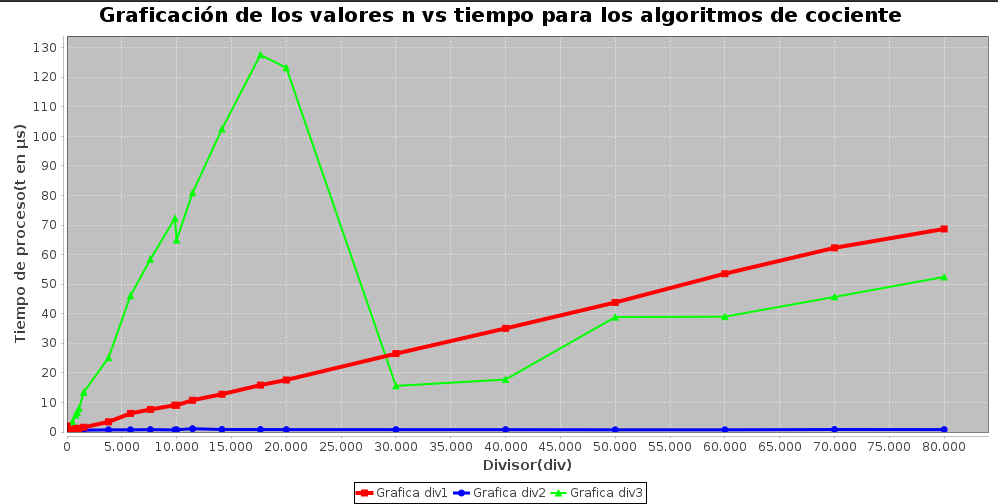
\includegraphics[width=20cm]{Imagenes/ResultadosExperimentalesCocientes.png}
                \caption{Gráficas de los puntos ordenados obtenidos del registro de tiempo de procesamiento para una n incremental en cada algoritmo de cociente de números enteros}
            \end{figure}
        \subsubsection*{Análisis Asintótico}
            Ahora realizamos la comparación de las complejidades obtenidas \textit{a priori} en la sección anterior, y el análisis \textit{a posteriori} observable con las gráficas.\\
            
            \hfill \break
            
            \textbf{Primer algoritmo}\\
                El primer algoritmo se muestra en la gráfica como una curva de color rojo, al igual que el algoritmo del producto. La tendencia de comportamiento es clara y consistente con los valores evaluados, se define su comportamiento por una recta.\\
                Se toma la complejidad calculada analíticamente en el análisis \textit{a priori} para este algoritmo, y se muestran las complejidades comparadas en la siguiente tabla:
                
                \begin{table}[h!]
                    \centering
                    \begin{tabular}{c | c}
                        Método análisis & Complejidad \\ \hline
                        \textit{A priori} & O(n)\\
                        \textit{A posteriori} & $O(n)$\\
                    \end{tabular}
                \end{table}
                
               Claramente su crecimiento es lineal y se concluye que: $div1 \in \Theta(n)$
            
            \hfill \break
            
            \textbf{Segundo algoritmo}\\
                El segundo algoritmo, de naturaleza iterativa, se representa con una curva de color azul. Una vez más, nos enfrentamos a una representación engañosa de la que necesitaremos el análisis \textit{a priori} para no afirmar erróneamente que su descripción es la de una constante.\\
                Se recupera una vez más, la complejidad calculada de forma analítica para el segundo algoritmo de divisiones, y se muestran las complejidades según el método en la siguiente tabla:
                
                \begin{table}[h!]
                    \centering
                    \begin{tabular}{c | c}
                        Método análisis & Complejidad \\ \hline
                        \textit{A priori} & O(1)\\
                        \textit{A posteriori} & $O(log(n))$\\
                    \end{tabular}
                \end{table}
                
                Advertido por el resultado obtenido para su algorimo inverso de los productos, su descripción no será la de una constante, pero la de curva de crecimiento algorítmico: $div2 \in \Theta(log(n))$
            
            \hfill \break
            
            \textbf{Tercer algoritmo}\\
                El último algoritmo se plantea de forma recursiva, su gráfica es la de un color verde y que también muestra un comportamiento errático como el algoritmo también recursivo para los productos. Tomando directamente en cuenta solo la tendencia de la gráfica para los valores mayores de \textit{n}, podría sugerirse que se llega a comportar con un crecimiento lineal. Se eliminan las opciones que podría describir su comportamiento por debajo del de \textit{div1}, que no llegaría a superar para valores mayores; Su comportamiento no podría ligarse al de una constante, ni a la de una función logarítmica ni de una raíz, por lo que nos queda otorgarle las cualidades de una función descrita por una recta.\\
                Finalmente se muestra la tabla comparando las 2 complejidades obtenidas de los 2 métodos:
                
                \begin{table}[h!]
                    \centering
                    \begin{tabular}{c | c}
                        Método análisis & Complejidad \\ \hline
                        \textit{A priori} & O(n)\\
                        \textit{A posteriori} & $O(n)$\\
                    \end{tabular}
                \end{table}
                
                Concluimos finalmente entonces, que para este algoritmo recursivo, su complejidad es: $div3 \in \Theta(n)$
                
        \subsubsection{Eficiencia de los algoritmos}
            Rápidamente determinanos el algoritmo más eficiente del conjunto utilizado. El algoritmo de \textit{div2}, tiene complejidad $\Theta(log(n))$, siendo la menor de entre los 3.
            Los 2 algoritmos restantes, una vez más tendrán la misma complejidad acotada por $\Theta(n)$, donde solo el manejo de las constantes nos determina, de la familia de rectas, cuál es la que los acota más justamente.\\
            Se recurre a la gráfica para comprobar las tendencias de ambos logaritmos, y se identifica, aún con el comportamiento errático de su contrincante, que la gráfica de \textit{div1} es la que seguirá creciendo con una pendiente mayor resultando en mayor tiempo de procesamiento y por lo tanto \textbf{menos eficientemente}.
\newpage
\section*{Conclusiones}
    \begin{tabular}{l l}
        \multirow{3}{*}{
\includegraphics[width=1.5cm]{Imagenes/imanol.jpg}} &  \\
        & \textbf{Rivero Ronquillo Omar Imanol}\\
        & \\
    \end{tabular}
    \vspace*{3\baselineskip}\\
    Al iniciar el análisis de algoritmos iterativos era sencillo concluir que aquellos que parecían tener una menor cantidad de lineas de código eran aquellos que potencialmente tenían una menor complejidad algorítmica, sin embargo, cuando se realizaba un análisis a profundidad (que probablemente no sea necesario para alguien con más experiencia en el cálculo de complejidades), no siempre era aquello que representaba inicialmente.
    
    Resulta particularmente interesante aplicar un análisis \textit{a priori} y \textit{a posteriori} en algoritmos que finalmente están diseñados para resolver el mismo problema, sin embargo, gracias al análisis pudimos comprobar de manera teórica y posteriormente, de forma experimental, la diferencia fundamental entre estos algoritmos: su complejidad. Para aquellos que su complejidad era mayor era claro experimentar un consumo de tiempo de ejecución mas elevado, escalando progresivamente cuando se realizaban pruebas para valores muy grandes o para aquellos que, por su propia definición, le provocan caer en su peor caso al algoritmo.
    
    Para estos algoritmos, una vez más queda claro que no hay que dejar engañarnos por las primeras impresiones. Aunque los algoritmos recursivos \textit{prod3} y \textit{div3}, considerablemente tenian una menor cantidad de líneas de código que sus contrapartes iterativas, en ningún caso probaron ser mejores. Aún así para algunos casos como los de \textit{prod2()} y \textit{div2}, fue necesaria la comparación de sus resultados experimentales con sus respectivos resultados teóricos, provocados por una representación engañosa.
    
    Finalmente, me queda comentar que aunque un algoritmo recursivo sea mucho más simple de definir, no siempre será la mejor solución posible del problema.
    \hfill \break
    \hfill \break
    
    \begin{tabular}{l l}
        \multirow{3}{*}{
\includegraphics[width=1.5cm]{Imagenes/lalo.jpg}}  &  \\
        & \textbf{Valle Mart\'inez Luis Eduardo} \\
        & \\
    \end{tabular}
    
    \vspace*{3\baselineskip}
    En la presente práctica se desarrollaron implementaciones a un mismo problema a través de ópticas algoritmicas distintas. Se introdujo la recursividad como otro de los recursos disponibles para solucionar problemas, con códigos más reducidos y que en algunos casos, ofrecen métodos más sofisticados y elegantes.
    
    Pero por tener una cantidad menor de líneas de codficación, esto implica directamente una disminución en la complejidad en su ejecución. Por esta razón se analizaron, utilizando ambos métodos, \textit{a priori} y \textit{a posteriori}, la eficacia de una alternativa recursiva, frente a la clásica solución iterativa.\\
    
    Se comprobaron además, las ventajas y limitaciones de un método con perspectiva del otro, presentando también que en conjunto permiten clarificar las dudas posibles existentes y complementarse para hallar una respuesta correcta. Mientras el analítico requiere una completa y clara comprensión del funcionamiento y flujo del algoritmo para identificar la complejidad de cada bloque que lo integra, en el método experimental, si bien esta ímplicita la comprensión del funcionamiento del algoritmo, no es una limitante para sugerir, a través de la comparación de la tendencia que muestran los datos recopilados con el comportamiento de crecimiento de los diferentes tipos de funciones, la complejidad de este.\\
    
    En el proceso de desarrollo no nos encontramos en fallas o errores que perjudicaran significativamente el avance en su elaboración, sin embargo, origen de un razonamiento poco minucioso, se habían generado originalmente, valores de prueba para la generación de las gráficas que no cumplían con su objetivo, mostrar el comportamiento cuando el valor \textit{n} crecía gradualmente. Este error fue facilmente corregido manteniendo el otro parámetro de ingreso a la función constante, y variando únicamente el que correspondía al parámetro analizado para su recolección.
    
    Los resultados que se esperaban en la sección experimental, se basaban en los obtenidos de teóricamente, de manera que el error explicado antes fue identificado de esta forma. Sin embargo al ser corregido, en su mayor parte, salvo algunos fragmentos con comportamiento errático que atribuimos a procesos internos del lenguaje y el sistema pero que no son directamente casuados por el algoritmo analizado, fueron congruentes con las expectativas generadas del análisis.
\newpage

\begin{thebibliography}{X}
    \bibitem{clase7}Luna,B.[Benjamín Luna].(2020, Octubre, 6). CLASE 7 - ANÁLISIS DE ALGORITMOS[Archivo de video]. Recuperado de https://www.youtube.com/watch?v=XFSsIYKG4IE
\end{thebibliography}
\end{document}
